\documentclass[12pt]{article}
\usepackage{../lecture}
\lecture{23}{SAT, NP, and NP Hardness}
\date{April 22, 2021}

\begin{document}
\maketitle

\section{The Satisfiability Problem (SAT)}

\subsection{Propositional Formulas}
\begin{itemize}
    \item \textbf{Literal}: a boolean variable $x_i$ or its negation $\neg x_i$.
    \item \textbf{Clause}: a disjunction of literals ($x_1 \lor x_2 \lor \neg x_4$).
    \item \textbf{Formula in Conjunctive Normal Form (CNF)}: a propositional formula which is a conjunction of clauses ($(x_1 \lor x_2 \lor \neg x_4) \land (x_2 \lor \neg x_3) \land x_5$).
    \item A formula $\varphi$ is a 3CNF, a CNF formula such that every clause has exactly 3 literals.
\end{itemize}

\subsection{Satisfiability}
\begin{itemize}
    \item Problem: SAT
    \begin{itemize}
        \item Instance: A CNF formula $\varphi$.
        \item Question: Is there a truth assignment to the variable of $\varphi$ such that $\varphi$ evaluates to true?
    \end{itemize}
    \item Problem: 3SAT
    \begin{itemize}
        \item Instance: A 3CNF formula $\varphi$.
        \item Question: Is there a truth assignment to the variable of $\varphi$ such that $\varphi$ evaluates to true?
    \end{itemize}
\end{itemize}

\subsection{SAT $\leq_P$ 3SAT}
\begin{itemize}
    \item To reduce from an instance of SAT to an instance of 3SAT, we must make all clauses contain exactly 3 variables.
    \item Basic Idea:
    \begin{itemize}
        \item Pad short clauses so they have 3 literals.
        \item Break long clauses into shorter clauses.
        \item Repeat the above till we have a 3CNF.
    \end{itemize}
\end{itemize}

\subsection{2SAT}
\begin{itemize}
    \item 2SAT can be solved in polynomical time (specifically, linear time).
    \item There is no known polynomial time reduction from SAT (or 3SAT) to 2SAT. If there was, SAT and 3SAT would be solvable in polynomial time.
\end{itemize}

\section{NP}

\subsection{P and NP and Turing Machines}
\begin{itemize}
    \item \textbf{P}: the set of decision problems that have polynomial time algorithms.
    \item \textbf{NP}: the set of decision problems that have polynomial time non-deterministic algorithms.
    \item Many natural problems we would like to solve are in NP.
    \item Every problem in NP has an exponential time algorithm.
    \item P $\subseteq$ NP
    \item Some problems in NP are in P (shortest path problem)
    \item Big Question: Does every problem in NP have an efficient algorithm? This is the same as asking whether P $=$ NP.
\end{itemize}

\subsection{Problems with No Known Polynomial-Time Algorithms}
\begin{itemize}
    \item Problems:
    \begin{itemize}
        \item Independent Set
        \item Vertex Cover
        \item Set Cover
        \item SAT
        \item 3SAT
    \end{itemize}
    \item There are of course undecidable programs (no algorithm at all) but many problems that we want to solve are of similar flavor to the ones above.
    \item Question: What is common in the above problems?
\end{itemize}

\subsection{Efficient Checkability}
\begin{itemize}
    \item The above problems share the feature of checkability.
    \item \textbf{Checkability}: For any YES instance $I_X$ of $X$, there is a proof/certificate/solution that is of length poly($\left| I_X \right|)$ such that one can efficiently check that $I_X$ is indeed a YES instance.
\end{itemize}

\subsection{Certificers}
\begin{itemize}
    \item \textbf{Certifier/Verifier}: an algorithm $C(\cdot, \cdot)$ for problem $X$ if the following two conditions hold:
    \begin{enumerate}
        \item For every $s \in  X$, there is some string $t$ such that $C(s, t) = \text{"yes"}$.
        \item If $s \notin X$, $C(s, t) = \text{"no"}$ for every $t$.
    \end{enumerate}
    \item \textbf{Certificate/Proof}: the string $t$.
\end{itemize}

\subsection{Efficient (Polynomial-Time) Certifiers}
\begin{itemize}
    \item \textbf{Efficient Certifier}: A certifier $C$ for problem $X$ if there is a polynomial $p(\cdot)$ such that the following conditions hold:
    \begin{itemize}
        \item For every $s \in X$, there is some string $t$ such that $C(s, t) = \text{"yes"}$ and $\left| t \right| \leq p(\left| s \right|)$.
        \item If $s \notin X$, $C(s, t) = \text{"no"}$ for every $t$.
        \item $C(\cdot, \cdot)$ runs in polynomial time.
    \end{itemize}
\end{itemize}

\subsection{Examples}
\begin{itemize}
    \item Independent Set
    \begin{itemize}
        \item Problem: Does $G = (V, E)$ have an independent set of size $\geq k$?
        \item Certificate: Set $S \subseteq V$.
        \item Certifier: Check $\left| S \right| \geq k$ and that there are no pair of vertices in $S$ connected by an edge.
    \end{itemize}
    \item SAT
    \begin{itemize}
        \item Problem: Does formula $\varphi$ have a satisfying truth table?
        \item Certificate: Assignment $a$ of 0/1 values to each variable.
        \item Certifier: Check each clause under $a$ and say "yes" if all clauses are true.
    \end{itemize}
    \item Composites
    \begin{itemize}
        \item Problem: Is the number $s$ composite?
        \item Certificate: A factor $t \leq s$ such that $t \neq 1$ and $t \neq s$.
        \item Certifier: Check that $t$ divides $s$.
    \end{itemize}
    \item Primes
    \begin{itemize}
        \item Problem: Is the number $s$ prime?
        \item Certificate: ?
        \item Certifier: ?
        \item This problem is not obvious.
    \end{itemize}
\end{itemize}

\subsection{Asymmetry in the Definition of NP}
\begin{itemize}
    \item Only YES instances have a short proof/certificate. NO instances need not have a short certificate.
    \item co-NP is where a short certificate exists if a short NO certicate exists.
\end{itemize}

\subsection{Nondeterministic Polynomial Time}
\begin{itemize}
    \item \textbf{Nondeterministic Polynomial Time} (denoted by NP): the class of all problems that have efficient certifiers.
    \item A certifier is an algorithm $C(I, c)$ with two inputs:
    \begin{itemize}
        \item $I$: instance
        \item $c$: proof/certificate that the instance is indeed a YES instance of the given problem.
    \end{itemize}
    \item $C$ can be thought about as an algorithm for the original problem, if:
    \begin{itemize}
        \item Given $I$, the algorithm guesses (non-deterministically) a certificate $c$.
        \item The algorithm now verifies the certificate $c$ for the instance $I$.
    \end{itemize}
    \item NP can be equivalently described using Turing machines.
\end{itemize}

\subsection{P $\subseteq$ NP}
\begin{itemize}
    \item For a problem in P, there is no need for a certificate.
    \begin{itemize}
        \item Consider problem $X \in$ P with algorithm $A$. We need to demonstrate that $X$ has an efficient certifier:
        \begin{itemize}
            \item Certifier $C$ on input $s$, $t$, runs $A(s)$ and returns the answer.
            \item $C$ runs in polynomial time.
            \item If $s \in X$, then for every $t$, $C(s, t) =$ "yes".
            \item If $s \notin X$, then for every $t$, $C(s, t) =$ "no".
        \end{itemize}
    \end{itemize}
\end{itemize}

\subsection{Exponential Time}
\begin{itemize}
    \item \textbf{Exponential Time} (denoted EXP): the collection of all problems that have an algorithm which on input $s$ runs in exponential time.
\end{itemize}

\subsection{If P $=$ NP}
\begin{itemize}
    \item Many important optimization problems can be solved efficiently.
    \item The RSA cryptosystem can be broken, no security on the web, no ecommerce.
    \item Creativity can be automated.
\end{itemize}

\section{NP-Completeness}

\subsection{"Hardest" Problems}
\begin{itemize}
    \item What is the hardest problem in NP? How do we define it?
    \item Hardest problem must be in NP.
    \item Hardest problem must be at least as "difficult" as every other problem in NP.
\end{itemize}

\subsection{NP-Complete Problems}
\begin{itemize}
    \item \textbf{NP-Complete}: A problem $X$ such that
    \begin{itemize}
        \item $X \in$ NP
        \item for any $Y \in \text{NP}, Y \leq_P X$
    \end{itemize}
    \item Suppose $X$ is NP-Complete. Then $X$ can be solved in polynomial time if and only if P $=$ NP.
    \begin{itemize}
        \item $\implies$ Suppose $X$ can be solved in polynomial time.
        \begin{itemize}
            \item Let $Y \in$ NP. We know $Y \leq_P X$.
            \item We showed that if $Y \leq_P X$ and $X$ can be solved in polynomial time, then $Y$ can be solved in polynomial time.
            \item Thus, every problem $Y \in$ NP is such that $Y \in P$; NP $\subseteq$ P.
            \item Since P $\subseteq$ NP, we have P $=$ NP.
        \end{itemize}
        \item $\impliedby$ Since P $=$ NP, and $X \in$ NP, we have a polynomial algorithm for $X$.
    \end{itemize}
\end{itemize}

\subsection{NP-Hard Problems}
\begin{itemize}
    \item \textbf{NP-Hard}: A problem $X$ such that for any $Y \in$ NP, we have that $Y \leq_P X$.
    \item An NP-Hard problem need not be in NP.
\end{itemize}

\subsection{Consequence of Proving NP-Completeness}
\begin{itemize}
    \item If $X$ is NP-Complete, solving $X$ implies P $=$ NP.
    \item We believe P $\neq$ NP, so $X$ is unlikely to be efficiently solvable.
    \item At the very least, many smart people before have failed to find an efficient algorithm for $X$. (This is a proof by mob opinion -- take it with a grain of salt.)
\end{itemize}

\subsection{Cook-Levin Theorem}
\begin{itemize}
    \item \textbf{Cook-Levin Theorem}: SAT is NP-Complete.
    \item We have to show SAT is in NP and that every NP problem $X$ reduces to SAT.
    \item Steve Cook won the Turing award for this theorem.
\end{itemize}

\subsection{Proving that a Problem $X$ is NP-Complete}
\begin{itemize}
    \item To prove $X$ is NP-Complete, show that $X$ is in NP and give a polynomial-time reduction from a known NP-Complete problem, such as SAT, to $X$.
    \item SAT $\leq_P X$ implies that every NP problem $Y \leq_P X$.
    \begin{itemize}
        \item $Y \leq_P$ SAT and SAT $\leq _P X$. Hence, $Y \leq_P X$.
    \end{itemize}
    \item Other NP-Complete problems include
    \begin{itemize}
        \item 3SAT
        \item Independent Set
        \item Vertex Cover
        \item Clique
        \item 3 Color
        \item Hamiltonian Cycle
    \end{itemize}
\end{itemize}

\subsection{Pictorial View}
\begin{itemize}
    \item[] \begin{center}
        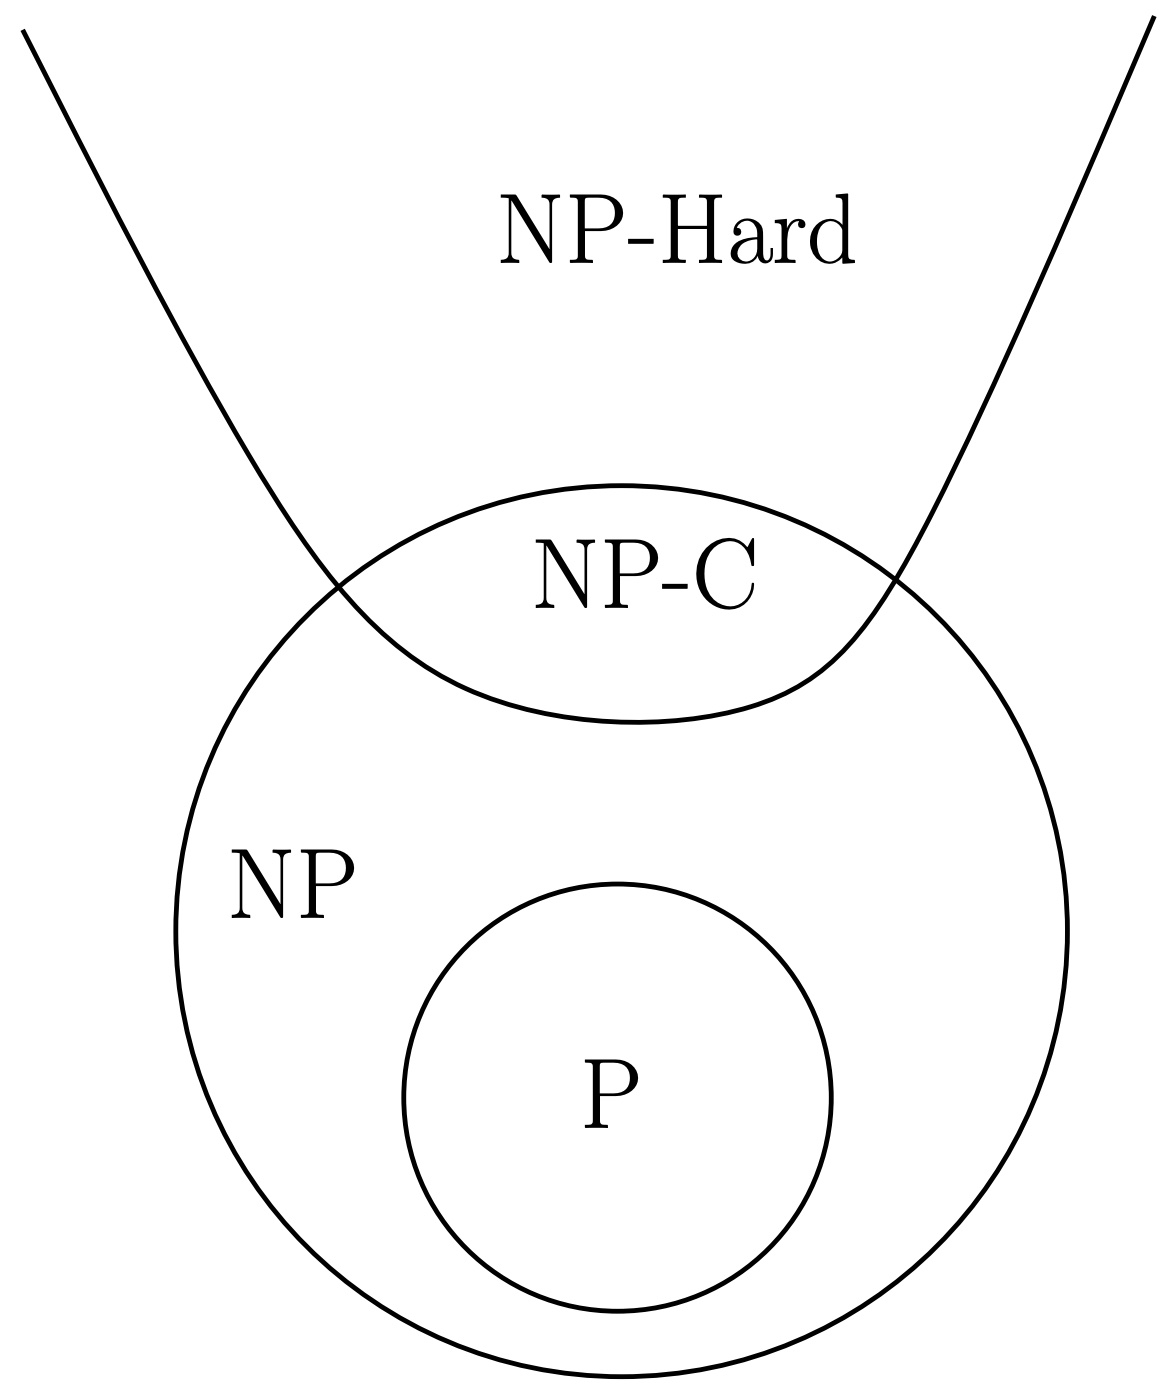
\includegraphics[width=0.4\textwidth]{images/p-np-complete-hard-diagram.jpg}
    \end{center}
\end{itemize}

\subsection{Ladner Theorem}
\begin{itemize}
    \item There are two possible scenarios: P $=$ NP and P $\neq$ NP.
    \item \textbf{Ladner Theorem}: If P $\neq$ NP, then there is a problem/language $X \in$ NP $\setminus$ P such that $X$ is not NP-Complete.
\end{itemize}

\end{document}
